\documentclass[11pt,a4paper]{article}

\usepackage[margin=1in]{geometry}
\usepackage{mathptmx}
\usepackage{amsmath}
\usepackage{amssymb}
\usepackage{amsthm}
\usepackage{braket}
\usepackage{tikz}
\usepackage{quantikz}
\usepackage{enumitem}
\usepackage{hyperref}
\usepackage{xcolor}

\definecolor{circuitblue}{RGB}{40,80,160}

\hypersetup{
    colorlinks=true,
    linkcolor=circuitblue,
    urlcolor=circuitblue,
    citecolor=circuitblue
}

\theoremstyle{definition}
\newtheorem{definition}{Definition}[section]
\newtheorem{example}{Example}[section]
\newtheorem{theorem}{Theorem}[section]

\theoremstyle{remark}
\newtheorem*{intuition}{Intuition}
\newtheorem*{keypoint}{Key Point}

\pagestyle{plain}

\setlength{\parindent}{0pt}
\setlength{\parskip}{6pt}

\begin{document}

\begin{center}
    {\LARGE \textbf{Quantum Feature Spaces and Kernels}}\\[8pt]
    {\large QML}\\[12pt]
    \hrule
\end{center}

\vspace{12pt}
\tableofcontents
\newpage

%% ========================================================
\section{Overview}
%% ========================================================

last lecture we saw that many VQCs r secretly linear classifiers in some quantum feature space. this lecture makes that precise: we develop the full theory of quantum feature maps, quantum kernels, and the connection to classical kernel methods. this is one of the cleanest and most important results in QML --- it gives us a principled way to understand wt quantum models actually compute, and when they might have an advantage.

the punchline: quantum computers naturally produce feature maps into exponentially large hilbert spaces, and the kernel trick lets us use these features without explicitly computing them. but (and this is the important part) having a big feature space doesnt automatically help --- the features need to be relevant to the task.

well cover the theory from the ground up, build the key circuits, and discuss the papers that shaped this field: havl\'i\v{c}ek et al. 2019 and liu-arunachalam-temme 2021.

%% ========================================================
\section{Classical Feature Maps and Kernel Trick (Deep Dive)}
%% ========================================================

we covered kernels briefly in lecture 08, but now we need the full picture.

\subsection{Feature Maps}

\begin{definition}[Feature Map]
a feature map is a function $\phi: \mathcal{X} \to \mathcal{F}$ that maps data from input space $\mathcal{X} \subseteq \mathbb{R}^d$ to a feature space $\mathcal{F}$ (a hilbert space, possibly infinite-dimensional).
\end{definition}

\begin{example}
polynomial feature map for $x \in \mathbb{R}^2$:
\[
\phi(x) = (1, x_1, x_2, x_1^2, x_1 x_2, x_2^2, x_1^2 x_2, x_1 x_2^2, x_1^2 x_2^2) \in \mathbb{R}^9
\]
maps 2D data into 9D. a linear classifier in this 9D space can represent quadratic decision boundaries in the original 2D space.
\end{example}

\begin{example}
gaussian (RBF) feature map: this one is infinite-dimensional!
\[
\phi(x) = e^{-\|x\|^2/2\sigma^2} \cdot \left(1, \frac{x}{\sigma}, \frac{x^{\otimes 2}}{\sigma^2\sqrt{2!}}, \frac{x^{\otimes 3}}{\sigma^3\sqrt{3!}}, \ldots\right)
\]
u cant compute $\phi(x)$ explicitly (infinite vector). but u CAN compute the inner product:
\[
\langle \phi(x), \phi(x') \rangle = e^{-\|x - x'\|^2/2\sigma^2}
\]
thats the kernel trick.
\end{example}

\subsection{The Kernel Function}

\begin{definition}[Kernel Function]
a kernel function $k: \mathcal{X} \times \mathcal{X} \to \mathbb{R}$ computes inner products in feature space:
\[
k(x, x') = \langle \phi(x), \phi(x') \rangle_{\mathcal{F}}
\]
\end{definition}

why this is powerful: if the feature space $\mathcal{F}$ is exponentially large (or infinite), computing $\phi(x)$ directly is intractable. but if we can evaluate $k(x,x')$ efficiently, we can do linear classification in that space without ever touching the full feature vector.

common classical kernels:
\begin{itemize}
    \item \textbf{linear:} $k(x, x') = x^\top x'$ (no feature map, just original features)
    \item \textbf{polynomial:} $k(x, x') = (x^\top x' + c)^d$ (degree-$d$ polynomial features)
    \item \textbf{RBF/gaussian:} $k(x, x') = e^{-\|x-x'\|^2/2\sigma^2}$ (infinite-dimensional feature space)
    \item \textbf{laplacian:} $k(x, x') = e^{-\|x-x'\|_1/\sigma}$
\end{itemize}

\subsection{Mercer's Theorem and Positive Semidefiniteness}

not every function $k(x,x')$ is a valid kernel.

\begin{theorem}[Mercer's Theorem (Informal)]
a symmetric function $k: \mathcal{X} \times \mathcal{X} \to \mathbb{R}$ is a valid kernel if and only if the kernel matrix (gram matrix) $K_{ij} = k(x_i, x_j)$ is positive semidefinite (PSD) for any finite set of points $\{x_1, \ldots, x_N\}$.
\end{theorem}

PSD means: for all $v \in \mathbb{R}^N$, $v^\top K v \geq 0$. equivalently, all eigenvalues of $K$ are non-negative.

the gram matrix for $N$ data points:
\[
K = \begin{pmatrix}
k(x_1, x_1) & k(x_1, x_2) & \cdots & k(x_1, x_N) \\
k(x_2, x_1) & k(x_2, x_2) & \cdots & k(x_2, x_N) \\
\vdots & \vdots & \ddots & \vdots \\
k(x_N, x_1) & k(x_N, x_2) & \cdots & k(x_N, x_N)
\end{pmatrix}
\]

\begin{keypoint}
any inner product in a hilbert space automatically gives a PSD kernel. this means: quantum feature maps $\phi(x) = \rho(x)$ with hilbert-schmidt inner product $\text{Tr}[\rho(x)\rho(x')]$ always define valid kernels. u dont need to check mercer's condition --- its guaranteed by quantum mechanics.
\end{keypoint}

\subsection{The Kernel Trick in Algorithms}

algorithms that depend on data only through inner products $\langle \phi(x_i), \phi(x_j) \rangle$ can be ``kernelized'':

\begin{itemize}
    \item \textbf{SVM:} dual formulation uses $k(x_i, x_j)$ --- the classic example
    \item \textbf{kernel ridge regression:} $f(x) = k(x, \cdot)^\top (K + \lambda I)^{-1} y$
    \item \textbf{kernel PCA:} eigendecompose the centered gram matrix
    \item \textbf{gaussian processes:} the kernel IS the prior covariance
\end{itemize}

%% ========================================================
\section{Quantum Feature Maps}
%% ========================================================

\subsection{The Basic Idea}

a quantum feature map encodes classical data $x$ into a quantum state:

\begin{definition}[Quantum Feature Map]
a quantum feature map is a map $\phi_Q: \mathcal{X} \to \mathcal{H}_{2^n}$ defined by:
\[
x \mapsto \ket{\phi(x)} = U_\phi(x)\ket{0}^{\otimes n}
\]
where $U_\phi(x)$ is a data-dependent unitary circuit and $\mathcal{H}_{2^n}$ is the $2^n$-dimensional hilbert space of $n$ qubits.
\end{definition}

with $n$ qubits, the state space is $2^n$-dimensional. thats exponential in the number of qubits:
\begin{center}
\begin{tabular}{c|c}
\textbf{qubits $n$} & \textbf{hilbert space dim $2^n$} \\
\hline
4 & 16 \\
10 & 1,024 \\
20 & 1,048,576 \\
50 & $\sim 10^{15}$ \\
100 & $\sim 10^{30}$
\end{tabular}
\end{center}

for comparison, the number of atoms in the visible universe is $\sim 10^{80}$. a 300-qubit feature map has more dimensions than atoms.

\subsection{Density Matrix Feature Map}

theres a subtlety: pure states $\ket{\phi(x)}$ have global phase ambiguity ($e^{i\alpha}\ket{\phi(x)}$ represents the same physical state). the more natural object is the density matrix:

\begin{definition}[Density Matrix Feature Map]
\[
x \mapsto \rho(x) = \ket{\phi(x)}\bra{\phi(x)} = U_\phi(x)\ket{0}\bra{0}^{\otimes n} U_\phi^\dagger(x)
\]
this lives in the space of $2^n \times 2^n$ hermitian matrices, which has real dimension $4^n$ (as opposed to $2^n$ for pure states).
\end{definition}

the feature space for density matrices is even bigger: $4^n$ real dimensions. for 10 qubits thats $\sim 10^6$ features. the inner product in this space is the hilbert-schmidt inner product:
\[
\langle \rho(x), \rho(x') \rangle_{HS} = \text{Tr}[\rho(x) \rho(x')]
\]

\subsection{Common Encoding Strategies}

lets go through the main quantum feature maps used in practice.

\textbf{1. angle encoding:}
\begin{center}
\begin{quantikz}
\lstick{$\ket{0}$} & \gate{R_Y(x_1)} & \qw \\
\lstick{$\ket{0}$} & \gate{R_Y(x_2)} & \qw \\
\lstick{$\ket{0}$} & \gate{R_Y(x_3)} & \qw \\
\lstick{$\ket{0}$} & \gate{R_Y(x_4)} & \qw
\end{quantikz}
\end{center}

each qubit encodes one feature as a rotation angle. feature space is a tensor product of 2D subspaces --- $2^n$ dimensional but highly structured. no entanglement means the quantum features r just products of single-qubit features. this is classically easy to simulate.

\textbf{2. ZZFeatureMap (havl\'i\v{c}ek encoding):}

for 3 qubits, 1 rep:
\begin{center}
\begin{quantikz}
\lstick{$\ket{0}$} & \gate{H} & \gate{R_Z(2x_1)} & \ctrl{1} & \gate{R_Z(\phi_{12})} & \ctrl{1} & \qw & \qw & \qw \\
\lstick{$\ket{0}$} & \gate{H} & \gate{R_Z(2x_2)} & \targ{} & \qw & \targ{} & \ctrl{1} & \gate{R_Z(\phi_{23})} & \ctrl{1} \\
\lstick{$\ket{0}$} & \gate{H} & \gate{R_Z(2x_3)} & \qw & \qw & \qw & \targ{} & \qw & \targ{}
\end{quantikz}
\end{center}

where $\phi_{ij} = 2(\pi - x_i)(\pi - x_j)$.

this creates entanglement through $ZZ$ interactions. the feature space includes cross-terms between features --- u cant decompose it into single-qubit contributions. this is the encoding that started the quantum kernel revolution.

\textbf{3. PauliFeatureMap (generalized):}

\[
U_\phi(x) = \prod_{\ell=1}^{r}\left[\exp\left(i\sum_{S} \phi_S(x) \bigotimes_{j\in S} P_j\right) H^{\otimes n}\right]
\]

the $S$ ranges over subsets of qubits, $P_j \in \{Z, Y, X\}$, and $\phi_S(x) = \prod_{j \in S} x_j$.

options:
\begin{itemize}
    \item $|S| = 1$, $P = Z$: ZFeatureMap (diagonal, no entanglement)
    \item $|S| \leq 2$, $P = Z$: ZZFeatureMap (pairwise entanglement)
    \item $|S| \leq 3$, mixed $P$: higher-order interactions, deeper circuits
\end{itemize}

\textbf{4. amplitude encoding:}
\[
\ket{\phi(x)} = \frac{1}{\|x\|}\sum_{i=0}^{2^n - 1} x_i \ket{i}
\]
encodes $2^n$ classical features in the amplitudes of $n$ qubits. exponentially efficient in space, but state preparation requires $O(2^n)$ gates in general.

\textbf{5. IQP-style encoding:}
\[
U_\phi(x) = \text{diag}\left(\exp(i f(x))\right) \cdot H^{\otimes n}
\]
where $f(x)$ is a polynomial in the features. IQP (instantaneous quantum polynomial) circuits r diagonal in the $Z$ basis. they r conjectured to be classically hard to simulate, which is important for quantum advantage.

\subsection{Encoding Strategies Compared}

\begin{center}
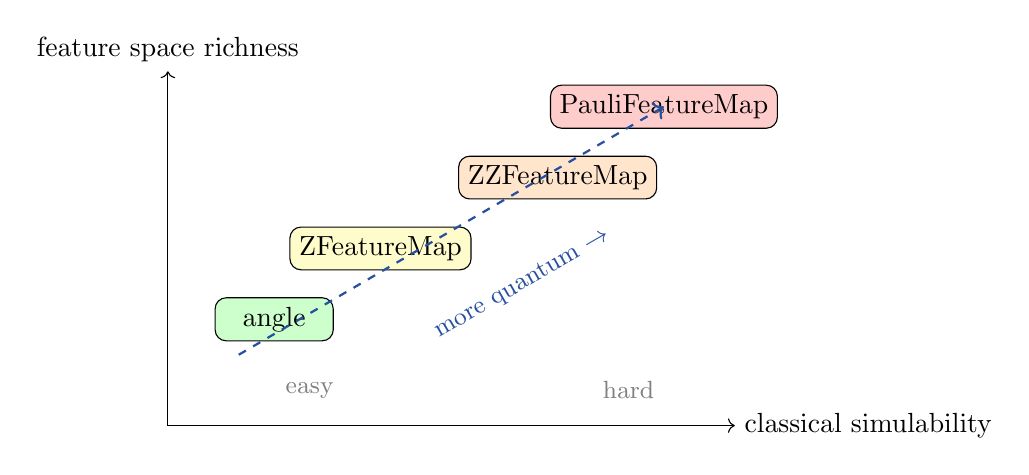
\begin{tikzpicture}[scale=0.9]
    % axes
    \draw[->] (0, 0) -- (8, 0) node[right] {classical simulability};
    \draw[->] (0, 0) -- (0, 5) node[above] {feature space richness};

    % encodings
    \node[draw, fill=green!20, rounded corners, minimum width=1.5cm] at (1.5, 1.5) (angle) {angle};
    \node[draw, fill=yellow!20, rounded corners, minimum width=1.5cm] at (3, 2.5) (z) {ZFeatureMap};
    \node[draw, fill=orange!20, rounded corners, minimum width=1.5cm] at (5.5, 3.5) (zz) {ZZFeatureMap};
    \node[draw, fill=red!20, rounded corners, minimum width=1.5cm] at (7, 4.5) (pauli) {PauliFeatureMap};

    % labels
    \node[gray] at (2, 0.5) {\small easy};
    \node[gray] at (6.5, 0.5) {\small hard};

    % arrow showing tradeoff
    \draw[->, thick, dashed, circuitblue] (1, 1) -- (7, 4.5);
    \node[circuitblue, rotate=30] at (5, 2) {\small more quantum $\to$};
\end{tikzpicture}
\end{center}

%% ========================================================
\section{The Quantum Kernel}
%% ========================================================

\subsection{Definition}

\begin{definition}[Quantum Kernel (Fidelity Kernel)]
the quantum kernel between two data points $x, x'$ is:
\[
\kappa(x, x') = |\braket{\phi(x)|\phi(x')}|^2 = \text{Tr}[\rho(x)\rho(x')]
\]
this is the transition probability (fidelity) between the two encoded quantum states.
\end{definition}

properties:
\begin{itemize}
    \item $\kappa(x, x) = 1$ for all $x$ (a state always has fidelity 1 with itself)
    \item $0 \leq \kappa(x, x') \leq 1$ (fidelity is bounded)
    \item $\kappa(x, x') = \kappa(x', x)$ (symmetric)
    \item the gram matrix $K_{ij} = \kappa(x_i, x_j)$ is PSD (its a valid kernel by mercer's theorem)
\end{itemize}

\begin{keypoint}
every quantum encoding circuit automatically defines a valid kernel. u dont need to check mercer's condition --- its guaranteed by the hilbert space inner product structure. this is a beautiful fact: the physics gives u the math for free.
\end{keypoint}

\subsection{Why the Fidelity?}

the quantum kernel $\kappa(x,x') = |\braket{\phi(x)|\phi(x')}|^2$ measures how ``similar'' the two encoded states are:
\begin{itemize}
    \item $\kappa = 1$: states are identical (same point in feature space)
    \item $\kappa = 0$: states are orthogonal (maximally different)
    \item $\kappa$ close to 1: data points are mapped nearby in hilbert space
    \item $\kappa$ close to 0: data points are mapped far apart
\end{itemize}

for classification: we want same-class points to have high $\kappa$ and different-class points to have low $\kappa$. if the feature map achieves this, a kernel SVM will find a good classifier.

\subsection{Computing the Quantum Kernel: The Overlap Circuit}

to compute $\kappa(x, x') = |\bra{0}^{\otimes n} U_\phi^\dagger(x') U_\phi(x) \ket{0}^{\otimes n}|^2$, we use this circuit:

\begin{center}
\begin{quantikz}
\lstick{$\ket{0}$} & \gate[3]{U_\phi(x)} & \gate[3]{U_\phi^\dagger(x')} & \meter{} \\
\lstick{$\ket{0}$} & & & \meter{} \\
\lstick{$\ket{0}$} & & & \meter{}
\end{quantikz}
\end{center}

apply $U_\phi(x)$ to prepare $\ket{\phi(x)}$, then apply the inverse $U_\phi^\dagger(x')$. if $x = x'$, this gives $U_\phi^\dagger(x)U_\phi(x) = I$, so we get $\ket{0}^{\otimes n}$ with certainty.

measure all qubits in the computational basis. the probability of getting the all-zeros outcome is:
\[
P(00\ldots0) = |\bra{0}^{\otimes n} U_\phi^\dagger(x') U_\phi(x) \ket{0}^{\otimes n}|^2 = \kappa(x, x')
\]

\begin{keypoint}
the kernel is estimated by running the overlap circuit many times and counting how often u get the all-zeros outcome. the fraction of all-zeros measurements gives $\hat{\kappa}(x,x')$.
\end{keypoint}

\subsection{Explicit Example: 2-Qubit ZZFeatureMap Kernel}

the overlap circuit for ZZFeatureMap on 2 qubits:

\begin{center}
\begin{quantikz}
\lstick{$\ket{0}$} & \gate{H} & \gate{R_Z(2x_1)} & \ctrl{1} & \gate{R_Z(\phi_{12})} & \ctrl{1} & \ctrl{1} & \gate{R_Z(-\phi'_{12})} & \ctrl{1} & \gate{R_Z(-2x'_1)} & \gate{H} & \meter{} \\
\lstick{$\ket{0}$} & \gate{H} & \gate{R_Z(2x_2)} & \targ{} & \qw & \targ{} & \targ{} & \qw & \targ{} & \gate{R_Z(-2x'_2)} & \gate{H} & \meter{}
\end{quantikz}
\end{center}

where $\phi_{12} = 2(\pi-x_1)(\pi-x_2)$ and $\phi'_{12} = 2(\pi-x'_1)(\pi-x'_2)$. this is the circuit from havl\'i\v{c}ek et al. 2019.

\subsection{Shot Budget for Kernel Estimation}

each kernel entry $\hat{\kappa}(x,x')$ is estimated from $S$ shots:
\[
\hat{\kappa}(x,x') = \frac{\text{number of all-zero outcomes}}{S}
\]

this is a binomial random variable with mean $\kappa(x,x')$ and variance:
\[
\text{Var}[\hat{\kappa}] = \frac{\kappa(1-\kappa)}{S}
\]

to achieve additive error $\epsilon$ with high probability: need $S = O(1/\epsilon^2)$ shots.

for the full kernel matrix of $N$ training points: need to estimate $\binom{N}{2}$ entries (symmetric matrix, diagonal is 1). total cost:
\[
\text{total shots} = O\left(\frac{N^2}{\epsilon^2}\right)
\]

\begin{example}
$N = 100$ training points, $\epsilon = 0.01$ accuracy per entry:
\[
\text{total circuits} = \frac{100 \times 99}{2} \times \frac{1}{0.01^2} = 4{,}950 \times 10{,}000 = 49{,}500{,}000
\]
thats $\sim 50$ million circuit executions. at 10,000 circuits/second on current hardware $\approx$ 83 minutes. this is the main scalability bottleneck of quantum kernel methods.
\end{example}

%% ========================================================
\section{The Full QML Kernel Workflow}
%% ========================================================

\subsection{Pipeline Diagram}

\begin{center}
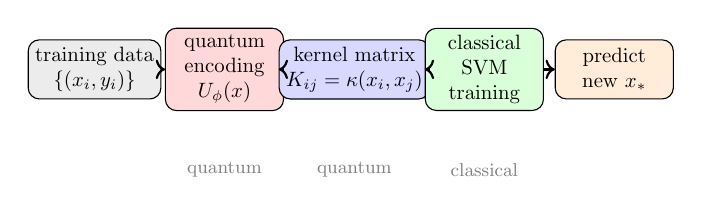
\begin{tikzpicture}[node distance=2.2cm, scale=0.75, every node/.style={scale=0.75}]
    \node[draw, rounded corners, fill=gray!15, minimum width=2cm, minimum height=1cm, align=center] (data) {training data\\$\{(x_i, y_i)\}$};
    \node[draw, rounded corners, fill=red!15, minimum width=2cm, minimum height=1cm, right of=data, align=center] (encode) {quantum\\encoding\\$U_\phi(x)$};
    \node[draw, rounded corners, fill=blue!15, minimum width=2.2cm, minimum height=1cm, right of=encode, align=center] (kernel) {kernel matrix\\$K_{ij} = \kappa(x_i, x_j)$};
    \node[draw, rounded corners, fill=green!15, minimum width=2cm, minimum height=1cm, right of=kernel, align=center] (svm) {classical\\SVM\\training};
    \node[draw, rounded corners, fill=orange!15, minimum width=2cm, minimum height=1cm, right of=svm, align=center] (pred) {predict\\new $x_*$};

    \draw[->, thick] (data) -- (encode);
    \draw[->, thick] (encode) -- (kernel);
    \draw[->, thick] (kernel) -- (svm);
    \draw[->, thick] (svm) -- (pred);

    % annotations
    \node[below of=encode, yshift=0.5cm, gray] {\small quantum};
    \node[below of=kernel, yshift=0.5cm, gray] {\small quantum};
    \node[below of=svm, yshift=0.5cm, gray] {\small classical};
\end{tikzpicture}
\end{center}

\subsection{Step by Step}

\begin{enumerate}
    \item \textbf{choose feature map:} pick $U_\phi(x)$ (ZZFeatureMap, PauliFeatureMap, etc.)
    \item \textbf{compute kernel matrix:} for all pairs $(x_i, x_j)$ in training set, run the overlap circuit and estimate $\kappa(x_i, x_j)$. result: $N \times N$ matrix $K$.
    \item \textbf{train SVM:} use $K$ as the kernel matrix in a classical SVM. this is a convex optimization problem --- no local minima, guaranteed global optimum. u get support vectors and dual coefficients $\alpha_i$.
    \item \textbf{predict:} for new point $x_*$, compute $\kappa(x_*, x_i)$ for all support vectors $x_i$. the prediction is:
    \[
    f(x_*) = \text{sign}\left(\sum_{i \in \text{SV}} \alpha_i y_i \kappa(x_i, x_*) + b\right)
    \]
\end{enumerate}

\subsection{Prediction Cost}

for a new test point $x_*$:
\begin{itemize}
    \item need to compute $\kappa(x_*, x_i)$ for each support vector $x_i$
    \item number of support vectors: typically $\sim 10$--$30\%$ of training set
    \item each kernel evaluation: $O(1/\epsilon^2)$ shots
    \item prediction cost per test point: $O(N_{SV}/\epsilon^2)$
\end{itemize}

%% ========================================================
\section{When Quantum Kernels Help vs When They Dont}
%% ========================================================

\subsection{The Two Conditions for Quantum Advantage}

\begin{keypoint}
a quantum kernel provides a genuine advantage only when BOTH conditions hold:
\begin{enumerate}
    \item \textbf{computational hardness:} the kernel $\kappa(x,x')$ cannot be efficiently computed classically
    \item \textbf{task relevance:} the kernel is useful for the classification task (high kernel-target alignment)
\end{enumerate}
either condition alone is insufficient. a classically hard kernel that doesnt separate the data is useless. a great kernel that can be computed classically needs no quantum computer.
\end{keypoint}

\subsection{When Quantum Kernels are Classically Simulable}

the quantum kernel is classically easy when:
\begin{itemize}
    \item \textbf{no entanglement:} tensor product encodings (angle encoding, ZFeatureMap). the kernel factorizes: $\kappa(x,x') = \prod_i \kappa_i(x_i, x'_i)$. each factor is a simple function.
    \item \textbf{clifford circuits:} gottesman-knill theorem --- clifford circuits can be simulated in polynomial time. if the feature map is clifford, the kernel is classical.
    \item \textbf{low entanglement:} if the entanglement entropy stays bounded, matrix product state methods can compute the kernel efficiently.
    \item \textbf{shallow circuits:} depth-$O(\log n)$ circuits with local gates can be contracted classically using tensor network methods.
\end{itemize}

\subsection{When Quantum Kernels Might Have an Advantage}

\begin{itemize}
    \item \textbf{deep entangling circuits:} ZZFeatureMap with multiple reps and all-to-all connectivity. these create long-range entanglement thats hard to simulate classically.
    \item \textbf{IQP-type encodings:} conjectured classically hard under standard complexity assumptions (polynomial hierarchy doesnt collapse).
    \item \textbf{specific problem structures:} problems with hidden algebraic structure (like discrete log) where quantum algorithms have proven advantages.
\end{itemize}

%% ========================================================
\section{Havl\'i\v{c}ek et al. 2019: The Foundation}
%% ========================================================

\subsection{The Paper}

``Supervised learning with quantum-enhanced feature spaces'' (Nature, 2019). this is THE paper that established quantum kernel methods.

\subsection{Key Contributions}

\begin{enumerate}
    \item defined the quantum kernel $\kappa(x,x') = |\braket{\phi(x)|\phi(x')}|^2$
    \item proposed the ZZFeatureMap encoding
    \item showed how to estimate the kernel on a quantum computer
    \item demonstrated it on a 2-qubit ibm quantum device
    \item proved that for certain data distributions, the quantum kernel provides a classification advantage
\end{enumerate}

\subsection{The Constructed Advantage}

havl\'i\v{c}ek et al. constructed a specific binary classification problem where:
\begin{itemize}
    \item the data is generated by a process related to the discrete logarithm
    \item the quantum kernel with ZZFeatureMap perfectly separates the classes
    \item any classical kernel with polynomial-dimensional feature space fails
\end{itemize}

\begin{intuition}
the idea is simple: design the dataset so that the ``correct'' decision boundary lives in a quantum feature space that classical models cant access. then the quantum kernel wins by construction.

the catch: this is an artificial dataset designed for quantum advantage. the open question is whether natural datasets have this structure.
\end{intuition}

\subsection{Experimental Results}

on 2 qubits (ibm device):
\begin{itemize}
    \item quantum kernel SVM: $\sim 100\%$ accuracy on the constructed dataset
    \item classical SVM (various kernels): $\sim 50\%$ (random guessing)
    \item this was one of the first experimental demonstrations of a quantum ML advantage
\end{itemize}

%% ========================================================
\section{Liu-Arunachalam-Temme 2021: Rigorous Advantage}
%% ========================================================

\subsection{The Paper}

``A rigorous and robust quantum speed-up in supervised machine learning'' (Nature Physics, 2021). this paper put the advantage on rigorous footing.

\subsection{Key Result}

\begin{theorem}[Liu et al. 2021 --- Informal]
there exist classification problems where:
\begin{enumerate}
    \item a quantum kernel method achieves high accuracy with polynomial samples and time
    \item any classical ML method (not just kernel methods --- ANY classical algorithm) requires superpolynomial resources
\end{enumerate}
the advantage holds under standard cryptographic assumptions (hardness of learning with errors).
\end{theorem}

\subsection{Why This Matters}

the havl\'i\v{c}ek result showed advantage over classical \textit{kernel methods}. liu et al. showed advantage over \textit{all classical methods}. thats a much stronger statement.

but: the problems are still artificial (based on cryptographic constructions). no one has shown this kind of advantage for a natural, practically relevant classification task.

\subsection{The Geometric Test}

liu et al. also introduced a practical diagnostic: the \textbf{geometric difference}:
\[
g(K_C, K_Q) = \sqrt{\left\|\sqrt{K_Q^{-1}} K_C \sqrt{K_Q^{-1}}\right\|_\infty}
\]

where $K_C$ is the best classical kernel matrix and $K_Q$ is the quantum kernel matrix.

\begin{itemize}
    \item if $g \gg 1$: the quantum kernel captures structure that the classical kernel misses. potential for quantum advantage.
    \item if $g \approx 1$: the two kernels are similar. no quantum advantage expected.
\end{itemize}

this gives u a practical test: before committing to quantum kernel methods, compute $g$ and check if its worth it.

%% ========================================================
\section{Kernel Concentration Problem}
%% ========================================================

\subsection{The Problem}

\begin{definition}[Kernel Concentration]
a quantum kernel exhibits concentration when:
\[
\kappa(x, x') \approx \delta_{x,x'} \cdot 1 + (1 - \delta_{x,x'}) \cdot \frac{1}{2^n}
\]
for most pairs $(x, x')$. that is, the kernel value for distinct points approaches $1/2^n \approx 0$.
\end{definition}

\begin{intuition}
in a $2^n$-dimensional space, random vectors are nearly orthogonal. if the feature map distributes points uniformly (like a random circuit would), all pairwise inner products are exponentially small. the kernel matrix approaches the identity matrix, which carries no information about data structure.
\end{intuition}

\subsection{Why It Happens}

for an $n$-qubit system, the hilbert space has $2^n$ dimensions. by concentration of measure:
\[
\mathbb{E}_{x \neq x'}[\kappa(x, x')] = O(2^{-n})
\]

this happens when:
\begin{itemize}
    \item the feature map is highly expressive (forms a 2-design or close to it)
    \item many qubits with deep entangling circuits
    \item the data fills the feature space somewhat uniformly
\end{itemize}

\subsection{Consequences}

if $\kappa(x,x') \approx 0$ for all $x \neq x'$, the gram matrix $K \approx I$. then:
\begin{itemize}
    \item the SVM has no structure to exploit --- all points look equally different
    \item the classifier essentially memorizes the training set (each point is its own support vector)
    \item generalization is terrible bcs the kernel provides no useful inductive bias
\end{itemize}

this is the kernel analog of barren plateaus: both r manifestations of ``too much quantum'' making the model useless.

\subsection{Solutions}

\begin{enumerate}
    \item \textbf{projected quantum kernels (huang et al. 2021):} project onto reduced density matrices instead of using the full state:
    \[
    \kappa_{\text{proj}}(x,x') = \exp\left(-\gamma \sum_i \|\rho_i(x) - \rho_i(x')\|_F^2\right)
    \]
    where $\rho_i(x) = \text{Tr}_{\bar{i}}[\rho(x)]$ is the reduced density matrix of qubit $i$.

    \item \textbf{fewer reps:} use ZZFeatureMap with 1 rep instead of 2+. less expressibility = less concentration.

    \item \textbf{bandwidth tuning:} scale the data: $x \to \gamma x$. smaller $\gamma$ means smaller rotations, less expressive feature map, less concentration.

    \item \textbf{fewer qubits:} use dimensionality reduction (PCA) to reduce features before encoding. fewer qubits = less concentration.
\end{enumerate}

%% ========================================================
\section{Connection to Barren Plateaus}
%% ========================================================

\subsection{The Unified Picture}

thanasilp, tangpanitanon, and coles (2024) showed that kernel concentration and barren plateaus r closely connected:

\begin{theorem}[Thanasilp et al. 2024 --- Informal]
if a parameterized quantum circuit exhibits a barren plateau (exponentially vanishing gradients), then the associated quantum kernel also concentrates (exponentially small off-diagonal entries).
\end{theorem}

\begin{keypoint}
barren plateaus and kernel concentration r two sides of the same coin. both come from the circuit being ``too expressive'' (too close to a 2-design). avoiding one helps avoid the other. the common fix: use structured, problem-aware circuits instead of random deep circuits.
\end{keypoint}

\subsection{The Expressibility-Utility Tradeoff}

\begin{center}
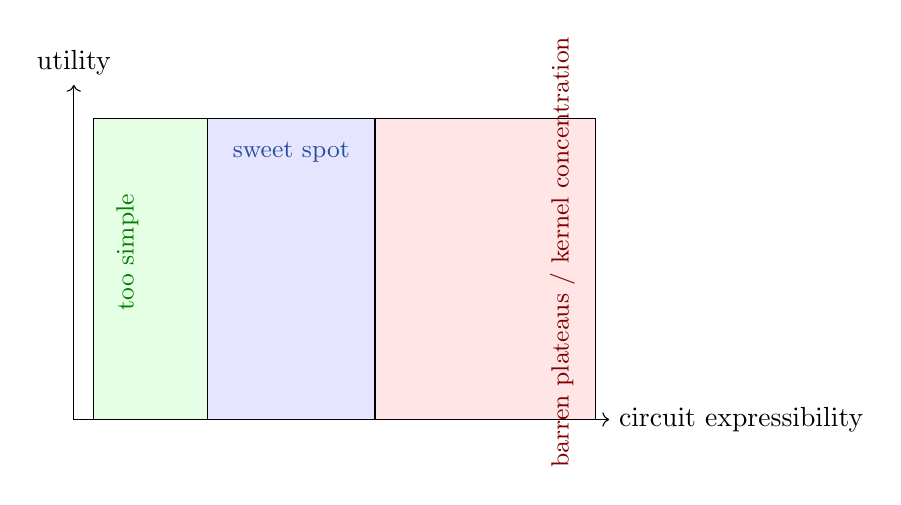
\begin{tikzpicture}[scale=0.85]
    \draw[->] (0,0) -- (8,0) node[right] {circuit expressibility};
    \draw[->] (0,0) -- (0,5) node[above] {utility};

    % curve
    \draw[thick, circuitblue, domain=0.5:7.5, smooth] plot (\x, {4*sin(\x*20)*exp(-0.15*(\x-3)^2) + 0.5});

    % too simple zone
    \draw[fill=green!10] (0.3, 0) rectangle (2, 4.5);
    \node[green!50!black, rotate=90] at (0.8, 2.5) {\small too simple};

    % sweet spot
    \draw[fill=blue!10] (2, 0) rectangle (4.5, 4.5);
    \node[circuitblue] at (3.25, 4) {\small sweet spot};

    % too expressive
    \draw[fill=red!10] (4.5, 0) rectangle (7.8, 4.5);
    \node[red!50!black, rotate=90] at (7.3, 2.5) {\small barren plateaus / kernel concentration};
\end{tikzpicture}
\end{center}

the sweet spot: expressive enough to capture task-relevant features, but not so expressive that the landscape becomes flat.

%% ========================================================
\section{Summary}
%% ========================================================

key takeaways:

\begin{enumerate}
    \item quantum feature maps encode classical data into $2^n$-dimensional (state) or $4^n$-dimensional (density matrix) hilbert spaces
    \item the quantum kernel $\kappa(x,x') = |\braket{\phi(x)|\phi(x')}|^2$ is always a valid kernel (PSD guaranteed by physics)
    \item computing the kernel requires the overlap circuit + measurement, with cost $O(N^2/\epsilon^2)$ for the full gram matrix
    \item the kernel workflow: encode $\to$ compute kernel matrix $\to$ train classical SVM $\to$ predict
    \item quantum advantage requires BOTH classical hardness AND task relevance
    \item havl\'i\v{c}ek et al. 2019 established the framework; liu et al. 2021 proved rigorous advantage (on artificial problems)
    \item kernel concentration: in large systems, kernels approach the identity matrix --- no useful structure
    \item kernel concentration and barren plateaus r two sides of the same coin (thanasilp et al. 2024)
    \item practical fixes: projected kernels, fewer reps, bandwidth tuning, dimensionality reduction
\end{enumerate}

the quantum kernel framework is theoretically beautiful and gives us the tools to rigorously analyze quantum ML models. but it also reveals the fundamental challenge: the exponentially large feature space is a double-edged sword.

next lecture: we put this theory into practice --- implementing quantum kernels in qiskit, computing kernel matrices, and running quantum SVMs.

\end{document}
